%% $RCSfile: proj_report_outline.tex,v $
%% $Revision: 1.2 $
%% $Date: 2010/04/23 02:40:16 $
%% $Author: kevin $

\documentclass[11pt, a4paper, twoside, openright]{report}


\usepackage{float} % lets you have non-floating floats
\usepackage{hyperref} % for typesetting urls
\usepackage{pifont}

\newcommand{\cmark}{\ding{51}}
\newcommand{\xmark}{\ding{55}}

%
%  We don't want figures to float so we define
%
\newfloat{fig}{thp}{lof}[chapter]
\floatname{fig}{Figure}

%% These are standard LaTeX definitions for the document
%%                            
\title{Security Visualisation Tools}
\author{Leliel Trethowen}

%% This file can be used for creating a wide range of reports
%%  across various Schools
%%
%% Set up some things, mostly for the front page, for your specific document
%
% Current options are:
% [ecs|msor]              Which school you are in.
%
% [bschonscomp|mcompsci]  Which degree you are doing
%                          You can also specify any other degree by name
%                          (see below)
% [font|image]            Use a font or an image for the VUW logo
%                          The font option will only work on ECS systems
%
\usepackage[image,ecs]{vuwproject}

% You should specifiy your supervisor here with
%     \supervisor{Firstname Lastname}
\supervisors{Ian Welch, Stuart Marshall}

% Unless you've used the bschonscomp or mcompsci
%  options above use
\otherdegree{Bachelor of Engineering(Hons)}
% here to specify degree

% Comment this out if you want the date printed.
\date{}

\begin{document}

% Make the page numbering roman, until after the contents, etc.
\frontmatter

%%%%%%%%%%%%%%%%%%%%%%%%%%%%%%%%%%%%%%%%%%%%%%%%%%%%%%%

%%%%%%%%%%%%%%%%%%%%%%%%%%%%%%%%%%%%%%%%%%%%%%%%%%%%%%%

\begin{abstract}

Detecting malicious attempts to access computers is difficult with current tools. Many current tools do not give the user the right information to find and analyse possible attempts. Visual analytics approaches support users to find the information they need. An effective visual analytics tool would improve detection rates.

\end{abstract}

%%%%%%%%%%%%%%%%%%%%%%%%%%%%%%%%%%%%%%%%%%%%%%%%%%%%%%%

\maketitle

%\chapter*{Acknowledgments}\label{C:ack} 
Any acknowledgments should go 
in here, between the title page and the table of contents.  The 
acknowledgments do not form a proper chapter, and so don't get a 
number or appear in the table of contents.

\tableofcontents

% we want a list of the figures we defined
\listof{fig}{Figures}

%%%%%%%%%%%%%%%%%%%%%%%%%%%%%%%%%%%%%%%%%%%%%%%%%%%%%%%

\mainmatter

%%%%%%%%%%%%%%%%%%%%%%%%%%%%%%%%%%%%%%%%%%%%%%%%%%%%%%%

% individual chapters included here
\chapter{Introduction}\label{C:intro}

Maintaining access control and information security has been an ongoing problem since people first realised that information is valuable and can be controlled. This problem quickly became apparent in networked systems after their invention and adoption outside the lab.

As networks have become ubiquitous and essential for modern life, threats to the integrity of networks and data have multiplied and diversified extensively. 
This proliferation of threats has lead to the design and use of tools intended to secure systems, and monitor for intrusions \cite{zhang2012survey}. Intrusions are defined loosely here as access to systems resources for purposes contrary to the intended use of the system, or access to the system by an unauthorised person (often an unauthorised person is also misusing the system). This may be as innocuous as browsing facebook while at work, or much more severe. Ie: stealing secrets or using the systems to run a botnet. Security policies exist as a formal statement of the intended uses of the system, and examples of uses considered malicious. The formal statement of acceptable and unacceptable system uses is extremely useful as it allows for configuring systems to deny many forms of intrusion. ie: denying remote login with an administrator account. 

There are two main forms of malicious user that should be considered. The outsider, these people do not have any legitimate access to the system. Obviously, their attempts should be denied. The second form is the insider attack. These may be significantly harder to detect as the attacker has legitimate access rights to the system, but is using them for purposes not authorised by the system owners.

Insider attacks are by far more difficult to combat effectively by technical means, as the user in question requires access to some or all of the systems to perform their jobs. This prevents simple solutions such as blanket denial of access. Further, this complicates detection of unauthorised access by obscuring illegitimate uses of the system within legitimate uses which should not be interfered with.

There are two main methods of operation for Intrusion Detection Systems(IDS).
Rule based systems, which flag any attempt that matches defined rules as malicious. These systems are extremely effective at detecting and blocking known attack patterns, particularly for outsider access as rules are relatively simple to write once the signature patterns in the attack are known. Insider attacks are more difficult to control with rules based systems, as blanket access blocks are often not suitable. 

Anomaly based detection systems use techniques from machine learning to automatically classify incoming events as normal or anomalous. Normal events are ignored, while anomalous events are flagged for operator attention. These systems have some obvious advantanges. Firstly they're able to recognise new intrusion methods, as they will appear as an anomaly, However, they're not able to provide much if any context for these events. Rule based systems at least identify which rule was matched. Anomaly detection systems are harder to disguise existing intrusions from, as their classification systems are flexible enough to recognise small changes in patterns. Rule based systems cannot do this as easily.

Both approaches are used heavily in monitoring network traffic generally. While somewhat successful, both approaches potentially suffer from false positives (Anomaly based more frequently than rules based) and possibly more worrying, false negatives. 

False negatives are quite obviously undesireable as each represents an intrusion that went undetected and potentially un-countered. Note that not all undetected intrusions will achieve their goals, however security administrators are not able to effectively ensure the vulnerabilities used are addressed, as they may remain unaware of the intrusion indefinitely, unless traces are left elsewhere in the system.

Large numbers of false positives are a serious problem for security systems as the quickly undermine user's trust in the systems \cite{stanton1994human}. Many IDS offer very limited forms of alerting with email most used, and SMS messaging an option for critical alerts. The limited range of sensory urgency available to IDS alerting mechanisms is problematic, as it causes a mismatch between the apparent and actual import of a message \cite{stanton1994human}. 

These factors leave a significant problem for security professionals. How do we ensure that actual intrusions are being detected, despite ever advancing intrusion techniques and rapidly growing size and complexity of networks to defend?. As I will show in Chapter \ref{C:back}, existing approaches fail to meet the goals laid out for this project. Many either do not scale well to large networks or easily cause information overload. Information overload creates an effect where the monitoring system looks a bit like a christmas tree. lots of pretty blinking lights, but no meaning. Many others fail to reveal important context about the events they flag. 

This project takes a data visualisation approach to solving the issue of detecting intrusion attempts, attempting to use human ability to spot and interpret novel patterns in data, without stripping context from the existing attempts. 

Due to time limitations, I will be restricting the focus of this tool from general network traffic, to remote access attempts through the SSH protocol. SSH is a commonly used protocol for server control and administration, as well as remote access and file sharing. ports used for SSH traffic are often the focus of intrusion attempts.

The overall goal is to create a tool that allows security adminstrators to effectively monitor remote access attempts to their systems for intrusions. 
In order to support this aim, several subidiary goals must be achieved.

\begin{enumerate}
\item{Clearly show patterns in login data.}
\item{Avoid information overload (the "christmas tree" effect).}
\item{Provide context for events.}
\item{Scale to many machines and millions of events.}
\end{enumerate}

Chapter \ref{C:back} discusses related works and reqirements for the project. Progress to date is discussed in chapter \ref{C:progress}, this is broken down into two major areas, design and evaluation. In chapter \ref{C:future} I discuss plans for the remaining work in three sections, Design, Implementation, and a timeline.

\chapter{Related Work}\label{C:back}

Much related work has been done in two major areas. Data mining focused techniques with visualisations used to explore the results of data mining, and visualisation driven techniques. Most visualisation driven techniques still contain significant datamining tools. Relatively little work has been done directly on access or system log visualisation, with research preferring to focus on network intrusion detetection logs. For the purposes of this section Intrusion Detection Systems(IDS) are treated as datamining systems. For anomaly based IDS this is straightforward, as they use traditional machine learning and datamining techniques to create classification systems for events. In rule based IDS, this is not so clear, as they apply pre-created rules. However, these rules are often created using data-mining techniques and serve to offer the same black box classification system as other data-mining software. I will be considering how each system discussed below meets the goals set out in Chapter \ref{C:intro}.

\subsection{Data Mining with Visualisation}

LogView \cite{4641277} is a visualisation tool designed to support undertstanding of information extracted through data-mining techniques applied to systems logs. The visualisation component uses treemaps to show clusters of events in a space efficient manner, with leaf nodes representing events, and branches showing clusters the events belong to. All leaf nodes are coloured in green, with shade darkening in 4 steps, representing  statuses OK, WARN, FAIL, OUTLIER in order.  The tool produced allows filtering based on time, and search terms. Time filtering shows only events occuring on the specified day in the map. Nodes matching search terms are highlighted red. Detailed information about a given event is available via mouseover. The simple filtering and interaction methods, coupled with very similar shades for clusters leaves the system very vulnerable to producing information overload in users. The overload potential grows rapidly as the logs grow, as there is very little information hiding present in this tool. 

\begin{figure}[tbh]
\fbox{\parbox[b]{.99\linewidth}{
\vskip 0.5cm
\centering 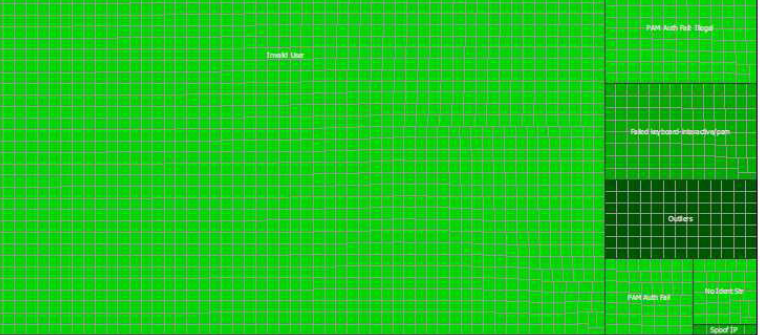
\includegraphics[scale=0.5]{tree.png}
\vskip 0.5cm}}
\caption{\protect\label{tree} LogView treemap of SSHD logs \cite{4641277}. Shades of green indicate severity of event.}
\end{figure}

A heirarchical system for visualising IDS logs \cite{itoh2006hierarchical} shows an interesting approach to the issue of context for IDS reports. Intrusion detection system messages are lacking in the context needed to support an evaluation of the priority and accuracy of the report. This tool shows the entire network under surveillance using a rectangle packing algorithm to group machines by subnets, the number of incidents sent and recieved from a given machine are displayed as a coloured bar rising out of the plane. This quickly leads to navigability and readability problems as the number of incidents reported grows. Simple filtering tools are available to limit by severity, time, IP and signature ID.
This system is highly reliant on an IDS system with both a low false positive, and false negative rate, as almost all information about the actual events is hidden, and no easy method to drill down to detailed information is provided.

A system log data mining approach is presented by W. Xu et al. \cite{Xu:2009:DLS:1629575.1629587}. This approach uses data mining and machine learning techniques heavily. Log syntax is automatically recovered through source code analysis, allowing the system to be applied to any source available software. Once log synatx is extracted, logs are parsed and machine learning algorithms used to perform feature extraction. Once the features were extracted the principle component analysis anomaly detection algorithm were applied to this data, to find interesting patterns in log messages. This approach identified many issues in the tested software, but was forced to be extended from a pure data-mining approach as users found the black box nature of data-mining algorithms caused difficulty in understanding why the results were as they are. To assist with this, a very simple decision tree visualisation was added, shown in Figure \ref{decision}. This visualisation was created with the intention of showing the logic used by the data-mining systems to give context for decisions. As the processing required for feature extraction and anomaly detection is highly parallel this approach readily scales to millions of entries, and shows very strong performance in detecting anomalous patterns in logs. However, from a security standpoint decision trees alone do not give sufficient context to easily determine if an anomaly represents an intrusion. This depends on much data not included in the raw logs.

\begin{figure}[tbh]
\fbox{\parbox[b]{.99\linewidth}{
\vskip 0.5cm
\centering 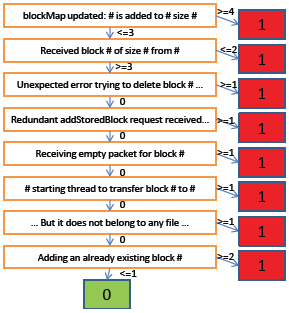
\includegraphics[scale=.75]{decisions.png}
\vskip 0.5cm}}
\caption{\protect\label{decision} Decision tree diagram \cite{Xu:2009:DLS:1629575.1629587}. Red 1's indicate anomalies, Green 0 indicates normal. labels on the edges show count thresholds for decisions.}
\end{figure}

\subsection{Visualisation Focused}

Picvis \cite{tricaud2008picviz} is a tool created to generate parallel co-ordinate plots of log data. Picviz offers tools to automate data extraction from several common log formats for use with their plot description language (pcl). This language allows a great deal of control over what variables are shown on a plot. Parallel co-ordinate plots can show strong clustering extremely well. However there are issues of scalability, as clusters and patterns can easily be hidden in background noise unless axes are well chosen. See Figure \ref{parallel}. Filtering tools are available to help address this limitation, but still require significant knowlege of the data structure and content. This tool would be excellent for confirmatory analyses however. 

\begin{figure}[tbh]
\fbox{\parbox[b]{.99\linewidth}{
\vskip 0.5cm
\centering 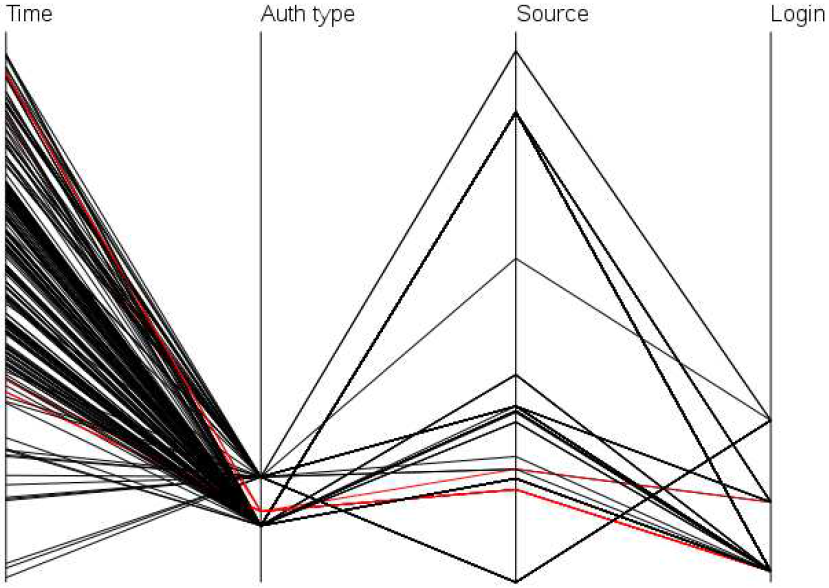
\includegraphics[scale=0.5]{parallel.png}
\vskip 0.5cm}}
\caption{\protect\label{parallel} Picviz parallel plots visualisation \cite{tricaud2008picviz} showing SSH logs.}
\end{figure}

Spiralview \cite{bertini2007spiralview} is a layout technique for timeseries data. Data is laid out in a spiral as shown in Figure \ref{spiral}. This technique has been used both for dynamic data streams \cite{chin2009visual} and analysis of static logs \cite{bertini2007spiralview}. In both applications strong promise is shown intially, as the spiral layout is intuitively expected to effectively reveal repeating patterns in time series data, such as intrusion detection system reports and access logs. However, the paper presenting the spiral technique for use in analysis of static logs does not attempt to evaluate the effectiveness with rigour \cite{bertini2007spiralview}. A rigorous evaluation of the spiral technique was performed in the paper proposing its use for dynamic datastreams \cite{chin2009visual}, However there are severe flaws in the presentation of this evaluation, as the table of results directly contradicts the text. 

\begin{figure}[tbh]
\fbox{\parbox[b]{.99\linewidth}{
\vskip 0.5cm
\centering 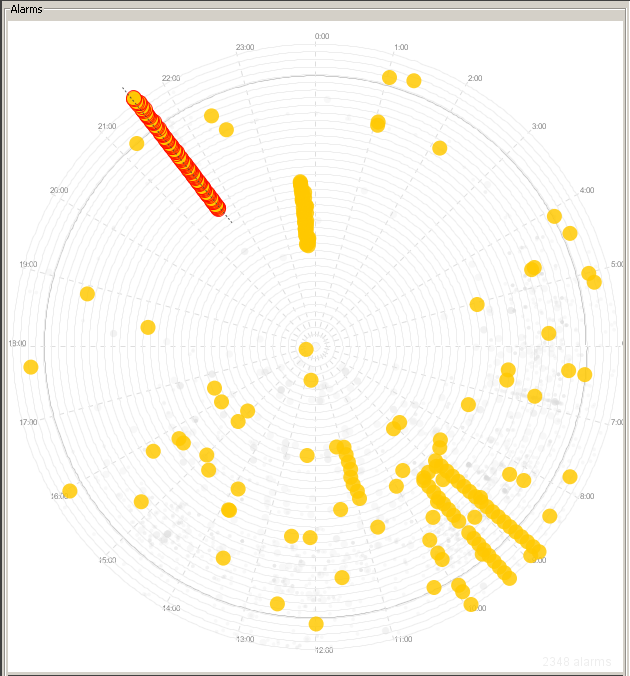
\includegraphics[scale=0.5]{spiral.png}
\vskip 0.5cm}}
\caption{\protect\label{spiral}Spiralview showing IDS logs over time. \cite{bertini2007spiralview}}
\end{figure}

Integrated visualisation system \cite{mukosaka2007integrated} is an IDS log based visualisation tool, focusing on attacks originating inside the monitored network, as these events are less well studied and have important security implications for the network. The tool provides a unified logical, geographic and temporal display of data, using three orthogonal planes. Multiple layouts of the three planes are available, with animated transitions. 

\begin{figure}[tbh]
\fbox{\parbox[b]{.99\linewidth}{
\vskip 0.5cm
\centering 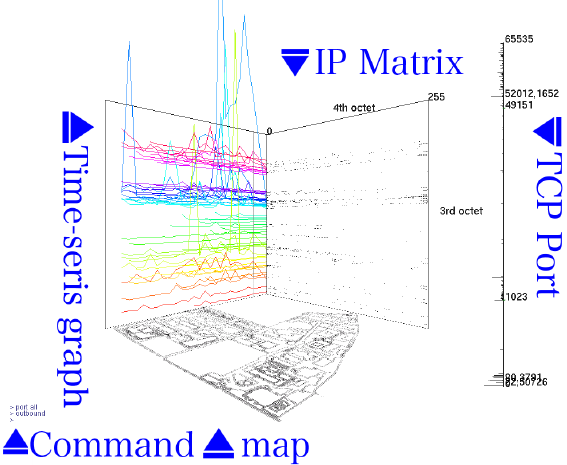
\includegraphics[scale=1]{integrated.png}
\vskip 0.5cm}}
\caption{\protect\label{integrated}Overview of integrated IDS visualisation system \cite{mukosaka2007integrated}. Newer events appear to the right of the time plane.}
\end{figure}

When in the configuration shown in Figure \ref{integrated}, the timeline plane shows events for the entire subnet x.y.x.*. Individual IP's can be chosen by shifting the timeline plane along the IP plane.
Filtering tools are made available to control what kinds of events are shown, though are not described in any kind of detail. port at least is usable to filter on. 

This system relies colour to distinguish ports on the timeline frame, which is easily subject to visual overload, as the human eye is not able to reliably distinguish fine differences in colours. Vertical position of the line indicates the number of events. With poorly described filtering systems and reliance on colour coding to distinguish ports, this system is extremely vulnerable to producing information overload. This leads to missing important events. the lack of data hiding creates visual clutter which can easily mask important intrusions composed of a small number of events. 

This system appears interesting as an attempt to correlate attack information with machine location through geoip systems. Where the number of events is "low enough" lines are drawn from IP plane to physical location on the lower plane. The exact number of lines drawn is not clear. 


\chapter{Project}\label{proj}

\section{Ethical Considerations}
Ethical issues arise solely around user evaluation.
As datasets are taken from real systems, these can contain real username, and possibly passwords (if mistakenly entered as username.)
\subsection{Datasets}
Honeynet dataset publically available. No futher anonymization is required for this dataset due to public availablity. if it's not properly anonymized, no further harm will be done. 

\subsection{Evaluation procedures}
Fairly standard for user evaluations. Privacy concerns, can't reveal identity of participants. 
Use numbers to refer to participants. destroy data after report completed. 

\section{User Personae}

\section{Requirements}\label{reqs}

In order to meet the goals laid out in Chapter \ref{C:intro} concrete requirements have been laid out for the tool.
These requirements are divided into functional and non-functional requirements. Requirements 1 through 3 and 6 support goals 1 and 2. Requirements 3 through 7 support goal 3. Scaling goals are supported by all requirements, as goals 1 and 2 strongly support scaling to millions of events.  

\begin{enumerate}
\item{Strong filtering and highlighting options.}
\item{Show surrounding context for anomalous accesses.}
\item{GeoIP support to add context to login attempts.}
\item{Allow the user control over which machine is monitored at any given time.}
\item{Show network context for currently monitored machine.}
\item{Extensible log parsing: don't prevent extension to other similar log types.}
\end{enumerate}

Non functional requirements deal with issues of performance, scalability and usability.
\begin{enumerate}
\item{Use information hiding to prevent information overload.}
\item{Prevent masking of important data.}
\item{Navigation: tool needs to support easy navigation of the timeline.}
\item{Performance capable of handling millions of events.}
\end{enumerate}

\section{Supporting tools}
Git -> distributed version control system. used to track code changes, and share codebase between uni and home. extremely useful as also provides multiple offsite backups (full codebase, with all revisions and comments are stored in each instance of the repository.)

GitHub -> site for sharing git repositories. Makes available an issue tracker which is integrated with git commit comments. Integration allows associating commits with issues, and closing issues from commits. this integration is extremely useful for debugging and tracking why changes were made. Issue tracker used heavily in later part of coding phase to track issues as detected, and link commits to problems resolved by that commit.
extremely helpful to keep thoughts organised and remember what issues exists. Also helpful for issue prioritisation.

Stack overflow -> (stackoverflow.com) Q\&A format website for assistance with programming issues. Extensive searchable database of questions with community feedback on answers has created an excellent practical reference for many languages, frameworks and libraries.  Extremely useful for finding out how to do things in an unfamiliar language. never actually had to ask my own question, as questions already answered and easily searchable.
\chapter{Design}\label{design}

I have chosen to implement a client server model for the system architecture, as this offers a strong separation into multiple loosely coupled modules. Given a client server architecture, and a desire for centralised data storage between multiple users a browser based approach was chosen. Using existing browsers leverages significant work done on secure network communications between client and server, as well as significant effort in sandboxing (isolating from the rest of the computer) in-browser applications. This saves significant time and effort on implementing communication protocols and security.  The client server model was chosen as typical users for the system are expected to be security professionals who can be expected to be required to document and report any abnormal behaviour. The client server model supports sharing the application amongst multiple users. 

As there are relatively few programming languages available for use within the browser this significantly simplified the choice of languages and tool sets. See section \ref{C:impl}.

\begin{figure}[tbh]
\fbox{\parbox[b]{.98\linewidth}{
\vskip 0.5cm
\centering 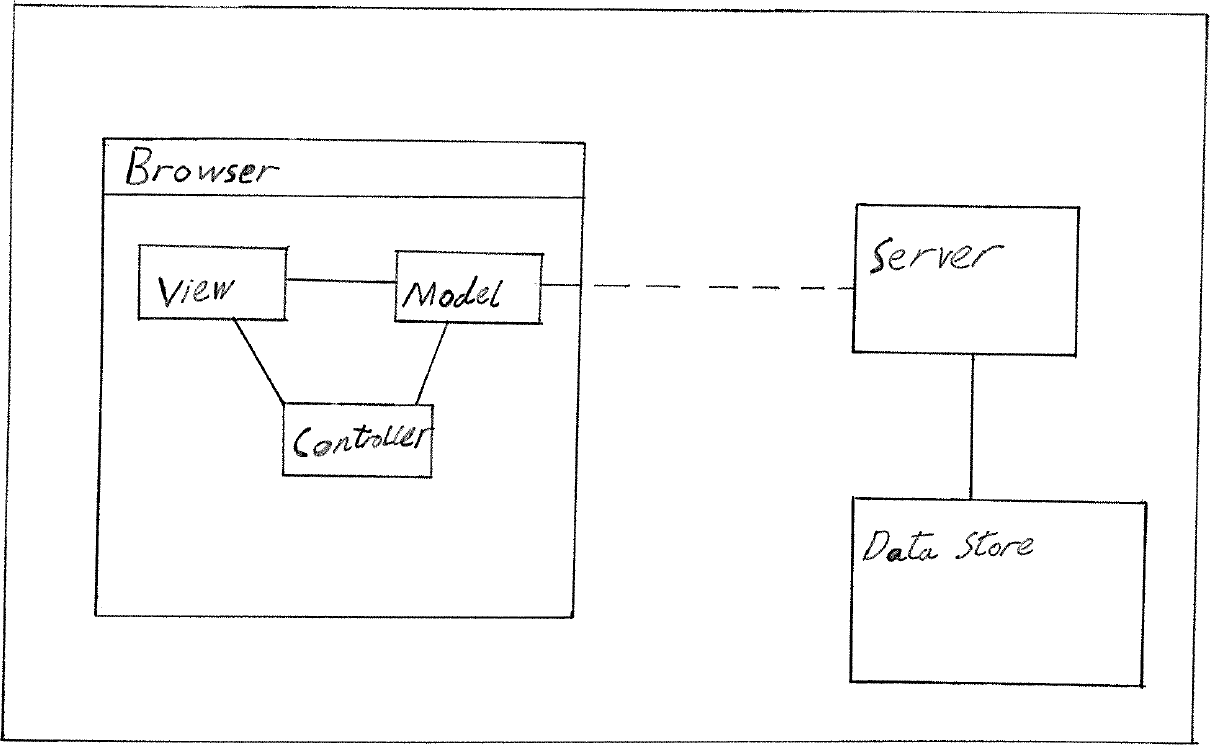
\includegraphics[scale=0.3]{blocks.png}
\vskip 0.5cm}}
\caption{\protect\label{spiral_plan}Block diagram showing proposed architecture of system. Note complete separation between server, browser and datastore. These may reside on separate machines.}
\end{figure}

Inside the browser there are three major components from an object oriented perspective. The view contains what is actually displayed on screen, this is implemented in HTML with SVG (Scalable Vector Graphics) for graphical components. The model stores the data and handles requests to the server as necessary. The controller is responsible for implementing user interaction with the system.

Communication between the client and server is handled through the HTTP protocol, using ajax requests.  The server software is responsible for serving data to the client, performing data aggregation, and limited data mining. In order to provide data, the server communicates with the data-store. This communication uses SQL and the JDBC api to interface with a database. Modular design permits creation of other storage interface modules. 

Data aggregation is performed server side for two reasons. In larger networks or over longer time periods many megabytes of logs can be created. While text is highly compressible this still creates significant network overhead to transfer. Further, there are unanswered questions about how well the client will perform with potentially millions of events to manipulate. Slow data transfers or interaction due to processing time would be a significant usability hurdle. Performing data aggregation on the server bypasses both of these limitations. 

\section{User interface design}\label{screen_design} 
  
I have chosen to adopt a time based approach for the visualisation elements, as access attempt logs have a very strong time component. Some forms of unusual behaviour are evidenced only by unusual times for access attempts, or unusual durations of access for example. Most existing visualisations do not give much emphasis to the time relation between access attempts, preferring to focus on the links between source and destination addresses. 

Two major approaches have been considered for displaying log entries.
Spiral view is an approach for displaying time series data mapped to a spiral, see figure \ref{spiral} where a straight line drawn from the outer edge to the center shows the same time at each level of the spiral \cite{bertini2007spiralview, chin2009visual}
These systems appear to be highly effective at displaying time series data in a fashion that supports easy detection of repeated patterns. 

\begin{figure}[tbh]
\fbox{\parbox[b]{0.98\linewidth}{
\vskip 0.5cm
\centering 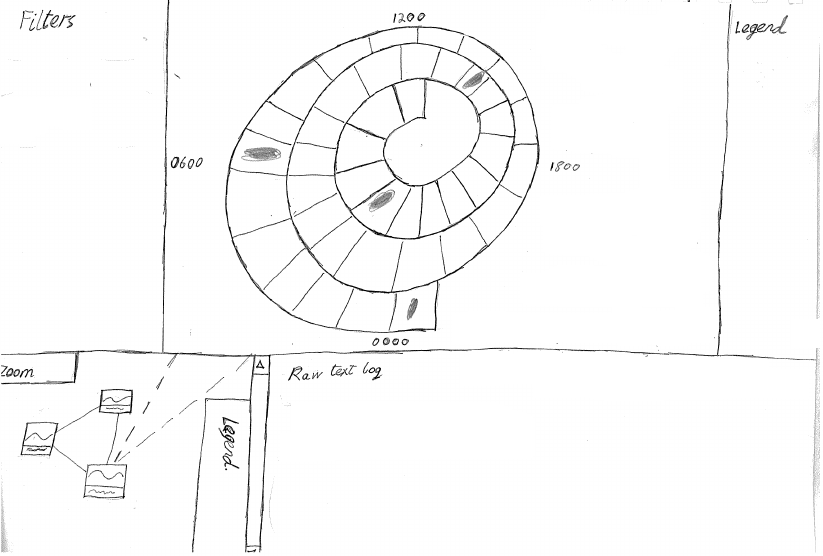
\includegraphics[scale=0.6]{spiral_plan.png}
\vskip 0.5cm }}
\caption{\protect\label{spiral_plan}Drawing showing proposed layout using spiralview for main focus. Black shading shows selection of an event with highlighting of related events.}
\end{figure}
 
However serious flaws in the results(\cite{chin2009visual}) of usability tests presented have lead to the rejection of this method. The error in question shows a table of results that directly contradict claims made in the text about how well spiralview supports the detection of patterns. The claims contradicted in the work are those directly bearing on the uses I had intended for the spiral layout. As this is a 300 hour project, I will not be attempting to repeat their work to clarify their findings. I attempted to contact the authors of the paper, and have as yet received no response.

This contradiction casts doubt on the ability of the spiralview model to effectively support data hiding, navigation and manage potential for information overload. These aspects are key functional requirements for this project \ref{reqs}. Due to this doubt, and lack of response from the authors when clarification was requested, I have chosen not to use the spiral model. 

\begin{figure}[tbh]
\fbox{\parbox[b]{.98\linewidth}{
\vskip 0.5cm
\centering 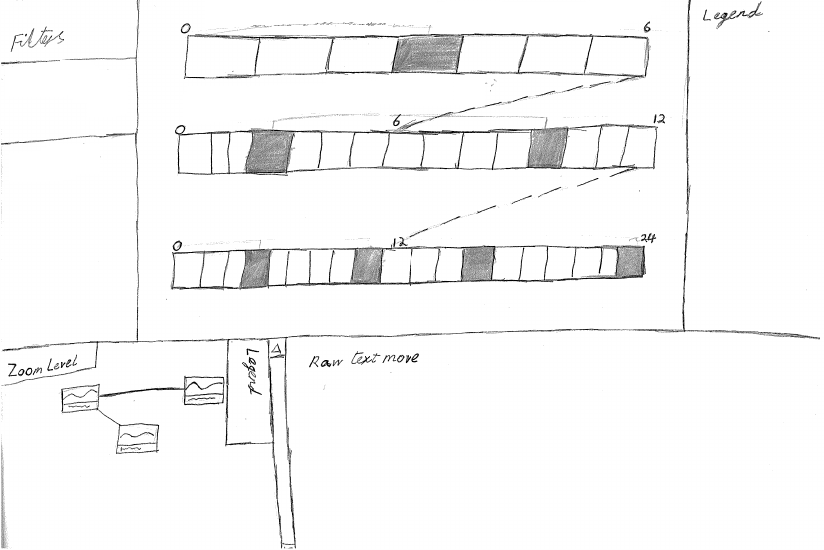
\includegraphics[scale=0.6]{lines.png}
\vskip 0.5cm}}
\caption{\protect\label{lines}Drawing showing proposed layout using multiple time lines for main focus. Black shading shows selection of an event, with highlighting related events.}
\end{figure}

Using block representation of data arranged linearly along a time axis.
Initial designs called for using a stacked representation where each layer represented twice the time of the previous layer. This is proposed to show patterns as an element that repeats a growing number of times in each layer.
Tufte's work on small multiples \cite{tufte1983visual} suggests keeping each level of the stack to represent the same amount of time, with differing start and end points. Ie: if the range is 6 hours, the top bar starts at 0600, and runs to 1200, the one below it from 0000 to 0600 and so on. This would show patterns repeating with a period less than the time range by showing in multiple bars. See Figure \ref{lines}. The timeline visualisation chosen is familiar to most people due to wide useage. Familiarity with this model supports information hiding and information overload prevention goals as users can be expected to interpret the timeline structure with minimal cognitive burden. 

I have been forced to consider data hiding techniqSues, as networks can become extremely busy, producing sufficient activity to overwhelm the user's ability to absorb information and detect meaningful patterns in the clutter. As I have chosen a time series based approach to displaying the data, I have chosen to use time binning to aggregate entities. This approach is extremely simple, with all entries in a short time period displayed as a single entity, with icons indicating some simple features of the hidden data. Such features include superuser accesses, abnormal numbers of failed access attempts, abnormally large numbers of access attempts, abnormal login locations for a user, abnormal login times for a user. Each time bin can be zoomed in on, allowing the user to see greater detail within the bin. For extremely busy systems and longer time periods there may be multiple levels of binning in play to aggregate sufficiently. This scheme reduces the visual complexity, while allowing easy access to detailed information about each incident. 

These last are the most complicated flags, as they require creating a profile of each user's access times over repeated access attempts. This complexity can produce false positives while the system is learning a new user's habits. and may be tripped up by a legitimate change in user habits.

\begin{figure}[tbh!]
\fbox{\parbox[b]{.99\linewidth}{
\centering 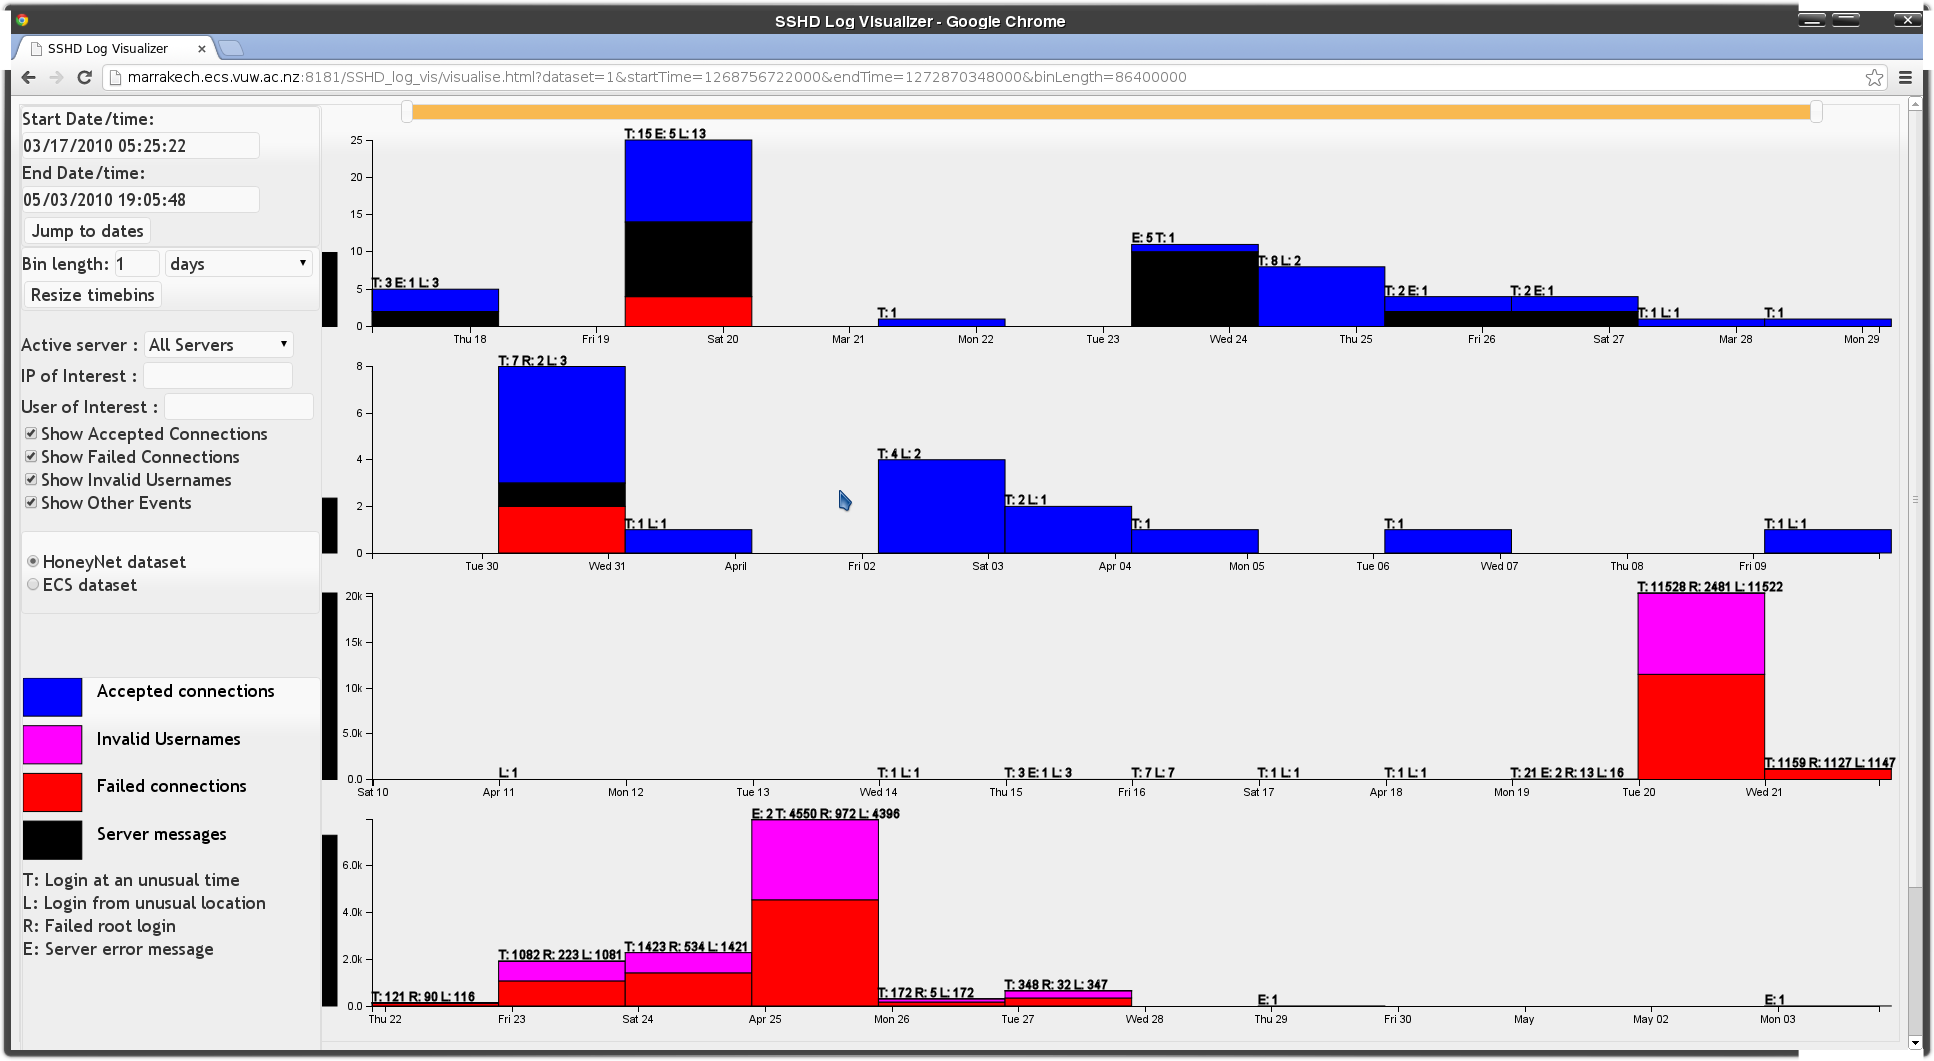
\includegraphics[scale=0.43,  angle=270]{screenshots/overview.png}
}}
\caption{\protect\label{overview}Tool showing overview of the honeynet dataset (\ref{data})}
\end{figure}

\subsection {Final design}

Figure \ref{overview} shows an overview of the tool produced. Network context and Raw line segments were ommitted (see \ref{lines}), These two components were considered less important than the timeline visualisations, and as such were dropped due to time pressures.  The space saved by dropping these components allowed more room in the left panel, which has absorbed the legend, allowing the remainder of the screen to be devoted to the timeline view. 

<IDK where to put this, but it certainly belongs in this subsection.>
All web application state is stored in the URL, and the application is capable of reloading the state from any correctly formatted URL. This was implemented to support uses expected from the user personae. It is reasonable to expect that a security officer would be required to log information about any detected anomalies, and may wish to obtain a second opinion.
With the tool able to reload state from a URL, this is easily supported simply by passing around the URL via existing collaboration tools, such as email. 
This also allows bookmarking of views that the user finds interesting, for later review or simply as way of saving current progress. 

Four notable features have been added since the design sketches were produced, vertical scaling; colour-coding of event types; mouseover tooltips; and a timeline overview. 
Within each timeline, blocks are vertically scaled proportional to the block with the largest number of events. Figure \ref{overview} demonstrates this most clearly in the first three blocks of the top timeline. The scale indicates 25 events at maximum, the first block consists of 5 events total, the second block is absent, indicating no events occured in that time, and the third block shows 25 events of three different classes. 

Timelines are required to have independent vertical scales as the number of events in a given time period may be highly variable. This is demonstrated in Figure \ref{overview} where the top timeline shows 25 events in the largest bin, and the third shows in excess of 20K events. Without independent scaling for each timeline all features of the upper two lines would be overwhelmed by the third. This lead to the inclusion of the black scale indicators found between the controls and timelines. They are logarithmically scaled such that the timeline with the highest maximum events per bin is represented by a full bar. These provide a quick visual indication of how much variability there is between scales. 

Each block is subdivided into four colours that represent 4 different classes of log event, as shown in the legend, Each event must be in exactly one event class, this allows the colour sections to be linearly scaled to block height easily (ie: if half the events are failed connections, half of the block will be red). These were added to give an instant overview of the approximate breakdown of event types within each bin, in support of requirements to avoid information overload without masking important data. To further support this goal hovering the mouse over a block produces a tooltip showing a detailed statistical breakdown of the events within that block (see Figure \ref{des_tooltip}). 

\begin{figure}[tbh]
\fbox{\parbox[b]{.99\linewidth}{
\centering 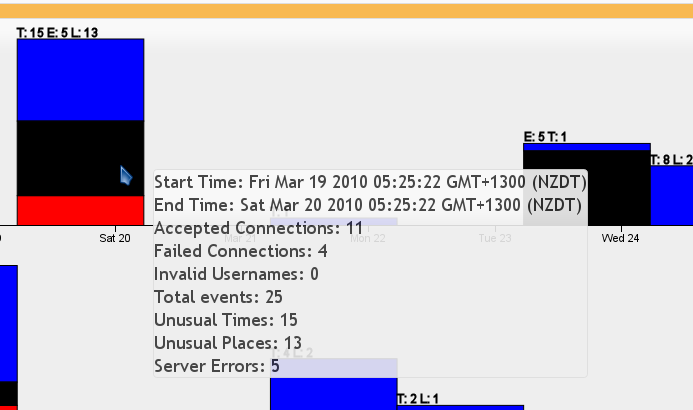
\includegraphics[scale=.35]{screenshots/overview_statistics_cropped.png}
}}
\caption{\protect\label{des_tooltip}Tooltip showing statistics for a block.}
\end{figure}

Above the timelines can be found a slider, when full (as in Figure \ref{overview}) this indicates that the timelines cover all data present. When there is more data off either end the slider shrinks to indicate how long a portion of the dataset is shown. The slider can then be dragged, and will move in steps, each step covering exactly as long as is currently shown in the timelines. Figure \ref{zoomed_in} demonstrates this shrinkage. 

\begin{figure}[tbh!]
\fbox{\parbox[b]{.99\linewidth}{
\centering 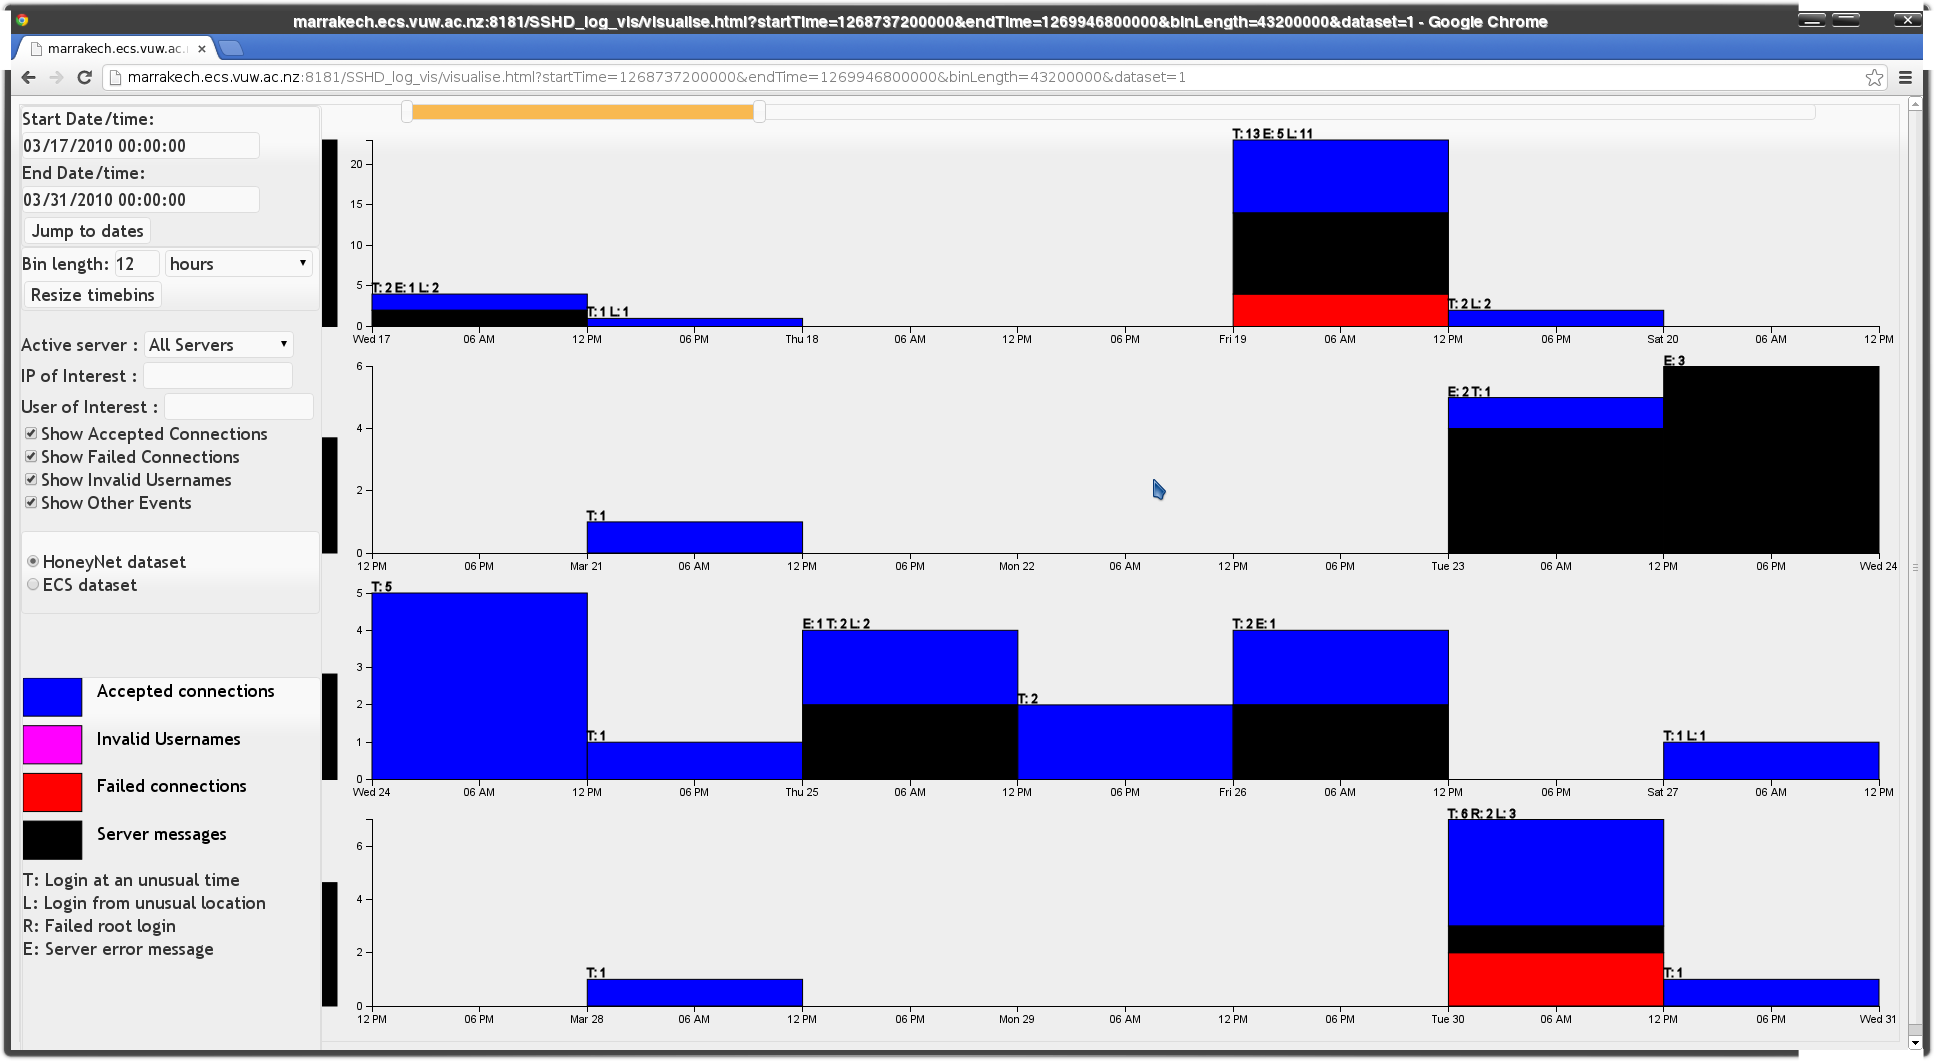
\includegraphics[scale=0.43,  angle=270]{screenshots/2_weeks_zoom.png}
}}
\caption{\protect\label{zoomed_in}Tool showing 2 weeks of Honeynet dataset (\ref{data})}
\end{figure}

Doubleclicking on any block zooms in on that block, with all four timelines reloading to show only data from the selected block. 
Zooming can be performed until either there is only one event in the chosen block, or each block covers 1 second. The one second limit is a practical consideration of the structure of SSHD logs. These logs have a time resolution of 1 second, ie:  all events occuring between 10:59:59.000 and 10:59:59.999 are logged at 10:59:59. Where there is only one event to display, mousing over the block will show the raw log line in a popup. This was implemented to reduce the number of zoom actions required to see details in low activity time blocks.

When there are multiple events in a 1 second block attempting to zoom will produce a popup dialog showing the raw log for that second (Figure \ref{des_one_second}).

\begin{figure}[tbh]
\fbox{\parbox[b]{.99\linewidth}{
\centering 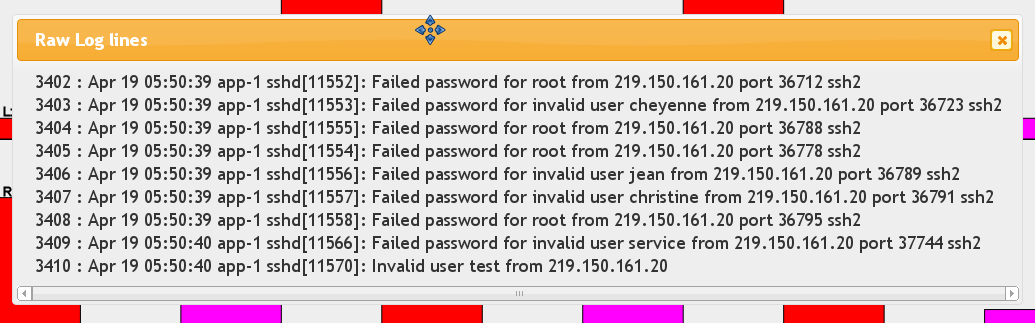
\includegraphics[scale=.35]{screenshots/single_second_popup.png}
}}
\caption{\protect\label{des_one_second}popup showing raw log for a single second.}
\end{figure}

This approach provides an arbitrarily large number of zoom levels, which supports information hiding goals.

No unzoom or undo functions were implemented. Instead the application was integrated with the browser history. This integration gives both undo and redo functions using the browser back and foward buttons. 

\section{Parser}\label{parser}

As SSHD logs are highly structured, this structure largely dictated the structure of the parser. There are 5 major classes of event that can be logged. While there are many more kinds of events, and metadata about connections that can be logged, extended information is highly dependent on SSH demon configuration. The listed message types can be relied on to be present in all useful logging levels. 
\begin{itemize}
\item{Connection attempts}
\item{Disconnection messages}
\item{Subsystem requests}
\item{Invalid usernames}
\item{System messages}
\end{itemize}

All log entries contain a partial timestamp, server name, service name and process id. These fields are required by the syslog format used by openSSH. The remainder of the message is a free text field. Each has different metadata to break down. IE:  a connection attempt has information about authentication method, username, source address, and status. Whereas a disconnection message contains a code, and source IP \ref{log_examples}.

The parser for SSH logs was initially conceived as a monolithic design, with a single class responsible for reading, analysing and writing data to the database. This design lasted into early implementation, where it was abandoned, as it leaves the parser too tightly coupled to the choice of underlying datastore. The parser was seperated into two layers, using a more abstract representation of each possible event type.

\begin{figure}[tbh]
\parbox{.99\textwidth}{
{\small Mar 16 08:25:22 app-1 sshd[4884]: Server listening on :: port 22. \\
Mar 16 08:25:22 app-1 sshd[4884]: error: Bind to port 22 on 0.0.0.0 failed: Address already in use. \\
Apr 19 05:55:20 app-1 sshd[12996]: Accepted password for root from 219.150.161.20 port 55545 ssh2 \\
Apr 19 05:55:20 app-1 sshd[12997]: Invalid user pauline from 219.150.161.20 \\
Apr 19 05:55:21 app-1 sshd[12990]: Failed password for root from 219.150.161.20 port 54890 ssh2 \\
Apr 20 00:00:51 app-1 sshd[24442]: subsystem request for sftp \\
Jun 8 01:03:34 machine0 sshd[1796]: Received disconnect from 38.165.101.19: 11: Bye Bye \\}}
\caption{Examples of SSHD logs, showing each type of message}
\label{log_examples}
\end{figure}

why do clustering here? - not really anywhere else to do it. Clustering in the server could only include data in current selection. This would result in instability in results (ie: if select one set of dates, a login is normal, select a different set and it's classified as abnormal). 

\section{Database} 

Why choose a RDBMS in the first place? maybe put this in the design overview section. Basically fell into RDBMS system because it's something I was somewhat familiar with in the beginning, and sufficiently appropriate.

Advantages of RDBMS systems, handle concurrency issues natively so long as transaction semantics are used, efficient filtering on attribute values. NoSQL datastores frequently do not handle concurrent access issues. This would require a significant redesign of both server and parser to handle concurrent updates. Concurrent reads present no issue. 

Schema for log events is represented in a single table \ref{entry_schema}. As there are several subtypes of log events, with differing metadata \ref{parser}, there are many nullable values in the event table.
\begin{table}[tbh]
\centering
\begin{tabular}{l || l | l | p{0.5\textwidth}}
Column & Datatype & Nullable & Conditions \\ \hline
id & Int & No & Autoincremented primary key \\
timestamp & Bigint & No & Timestamp stored as milliseconds since unix epoch. \\
server & int & No & Foreign key, linking to server table. \\
connid & int & No & Badly named, Process id for handling sshd process. \\
reqtype & Enum & No & Tag field, used to identify which of the possible event types this row represents. (connect, disconnect, subystem request, invalid username, other) \\
authtype & Enum & Yes & What authentication method was used. (password, hostbased, key, gssapi, or none) \\
status & Enum & Yes & Did the connection attempt succeed? (accepted, failed) \\
user & int & Yes & Foreign key to user table. \\
source & char(45) & Yes & text representation of Ipv4 or IpV6 address the request originated from. \\
port & smallint & Yes & Port the request was sent from. \\
subsystem & Enum & Yes & Which subsystem was requested. (sftp, scp) \\
code & int & Yes & disconnect code, not actually used. \\
isfreqtime & int & Yes & Reference to information about time cluster this request belongs to, or null. \\
isfreqloc & int & Yes & Reference to information about location cluster this request belongs to, or null. \\
rawline & text & No & Unprocessed line, exactly as read from logfile. \\
\end {tabular}
\caption{Schema for entry table}
\label{entry_schema}
\end{table}

Several considerations were involved in creating this table schema. As there are multiple types of log entry considered by the system, database design suggests three alternative approaches to table layout to handle this. A single unified table, with many nullable elements, A table storing all columns common to each entry type (Non nullable columns in \ref{entry_schema}) with additional tables for each subtype storing only information unique to that entry type. Or a table for each entry type with all attributes used in that subtype, including shared attributes.

It is usually considered good design to avoid large numbers of nullable attributes, as this complicates integrity checking and in many cases forces checks to be carried out at the application level, or in complex stored procedures. However, performance considerations have forced the use of this schema design. In practice, there are very few queries to the database that do not involve a range select on timestamp (all rows with timestamp between x and y) for all subtypes of entry. In both multitable schema designs, this must be implemented with multiple joins (5 or 6). As this tool is intended to scale to many millions of events, and joins are the least efficient database operation, nonfunctional requirements strongly suggest avoiding joins where possible. This has lead directly to the table schema shown \ref{entry_schema}. Note that the server table stores some basic metadata about each server, this is currently not utilized, though may be in future extensions.

The user table is a holdover from an older design<reword, it's actually necessary to link tables together.>, which proposed storing some metadata about users, such as validity, role, and login patterns. This would have eliminated the need for the invalid user request type, as this is just a failed connection, due to invalid user. This design was not pursued, due to issues with time. In the honeynet dataset, users are created and destroyed. This results in previously invalid usernames becoming valid. With this design, that would require multiple entries for each user, as an invalid user linked against an entry on date x, does not become valid when the user is created on date y (y after x).

Users may also have several independent frequent login times and locations, ie: Some IT staff may frequently log in from home as well as in the office. This resulted in frequent time and location information being split into four separate tables. <include table schema here?>

\section{Server}
Server implementation was very tightly constrained by choice of platforms. Web applications communicating through the HTTP protocol, with a Tomcat server provide limited opportunities for design choices.
In order for the code to interface with Tomcat, it must be written as at least one class which implements HttpServlet from the java API. 
This class serves to handle communication with the Tomcat server. Tomcat provides HTTP request parsing, session tracking and multithreading. Further classes may be used freely to implement servlet behaviour. As very simple behaviour is required from the server, I chose to use a two layer architechture for each Servlet. 
\begin{itemize}
\item{Data access layer. Responsible for fetching data from the underlying datastore. easily replaced to communicate with different kind of datastore. Takes values from client communication layer, returns lists of matching log entries.}
\item{Client Communication layer. Responsible for aggregating data returned by the data access layer, and building HTTP responses from the aggregated data. Including JSON translation.}
\end{itemize}
The data access layer is common to all servlets, and has a defined interface, with methods for fetching data to satisfy each type of request. This design allows for substitution of a different data storage system with minimal changes to the system. Servlets would need to be modified only to instantiate the new data access layer when initialised. This could be easily modified to use a static factory method, which would further restrict the area requiring changes.

There are exactly 4 types of request that may be made of the server, The majority of requests made in normal usage will be requests for aggregated events. 
\begin{itemize}
\item{Request aggregated events between given timestamps, and optional filters on username, server, and source IP}
\item{Request raw events between given timestamps, and optional filters on username, server, and source IP}
\item{Request start and end timestamps}
\item{Request list of all servernames}
\end{itemize}

These four requests to the server, are implemented with three requests to the underlying datastore.

\begin{itemize}
\item{Fetch log lines - used to fetch all log lines between a given pair of timestamps, with optional filters on username, server, and source IP}
\item{Fetch start and end times - used to fetch the timestamps of the first and last events in the datastore}
\item{Fetch all server names - used to fetch a list of every server name known to the datastore}
\end{itemize}

All request types are independent servlets within the web application. Each servlet has no shared state, so parallelizes easily within the tomcat framework. Connection pooling is implemented to assist in performance where multiple users may be requesting data. Concurrent read/write issues are the responsibility of the underlying datasource.

The first two request types use the same interface to the datasource, but have differing post processing applied. raw does not do any agreggation, simply converts the data into JSON format and embeds in the HTTP response. aggregated collects statistics about all events which fall in that time period, statistics are transmitted in JSON format as payload of HTTP response.
Why have aggregated request? nonfunctional requirements - performance and data hiding. aggregation done serverside due to bandwidth and memory requirements, this operation could involve processing millions of nodes for larger logs. This is unreasonable to send across the network in raw form, due to size and space requirements. Server has resources to do aggregation. 
some room for refactoring, this could be split into two layers
however the processing is quite simple, and only done for this one request type, so a data analysis layer was omitted.

\subsection{Security}

The database will contain a significant amount of privileged information about network security such as machine names and addresses, valid account names, and authentication methods used in the system. This data would be extremely useful to malicious users or outside intruders. 

As the tool is accessed through the browser there are concerns about the security of this information. As implemented, the tool does not directly include any authentication or access control mechanisms. However, the server is written to be resistant to SQL injection attacks through rigorous input sanitation.

This leads to a need to ensure that access to this tool is controlled through a robust authentication system. Ideally the web server hosting the tool should not be accessible to the outside world at all. Further, access should be restricted tightly to only those users with a definite need to have access. Secured connections must be used for all communication between client and server to limit the opportunity for malicious individuals to snoop on the data in transit. Tomcat natively supports access controls on a per application, or per page basis. Tomcat also supports SSH connection, and can be configured to require SSH connections on a per page or per app basis. These controls are managed through tomcat configuration files. 

Client side code contains no data, and so does not require security, as the server should deny access without valid credentials.
\chapter{Implementation}\label{C:impl}

\section{UI Implementation}\label{imp_ui} 

I have chosen to use javascript with the d3 visualisation library \cite{bostock2011d3} for the client portion of the system. This was chosen as d3 is a very well supported visualisation library offering excellent support for dynamic data, animations, graph layouts and highly customisable charting. Javascript, in addition to being required for D3, is the de-facto standard for interactive web applications. 
In addition JQuery and JQuery ui were used, as these frameworks allow for consistent behaviour across many different browsers, by abstracting away the cross browser support code into the framework. Further, JQuery offers significant support for DOM manipulation in simple and powerful ways. JQueryUI provides implementations of many common desktop UI widgets in forms suitable for web browsers (Javascript, HTMLand css). These widgets greatly simplified UI development, as they can simply be dropped in place and used. JQueryUI also provides CSS files and tools allowing easy tweaking or theming of the tool.
While this required learning a new language, javascript is a relatively simple language, and this did not pose a significant difficulty. Learning javascript was made significantly easier by extensive documentation and familiar syntax and somewhat familiar semantics. 

Filtering functions are currently somewhat limited, with options to show only data for a given username, IP addres, and toggle the display of each class of event. These filters can be freely combined. IP and username filters support wildcards, \_ matches a single character, \% matches 1 or more characters. 

This is a purely visual change, with no change in data, this can be seen as mousing over the bins shows the same summary information. These filters were implemented without altering the selected data to support exploration of potential attacks. ie: when looking for a brute force attack against root, I would hide failed attacks, as there are vastly fewer successful root logins, Then use the mouseover breakdown to check which (if any) bins had a suspiciously high failure rate. This would not be possible were the data to be filtered on the server side, as currently implemented the statistical summary would lose details.

Both date boxes are linked to datepicker tools, which allow for chosing a date from a calendar, and setting time through sliders. These values may be freely edited without reloading data. The Jump to dates button will trigger a reload of data. 
Binlength (Immediately below date controls) allows chosing the length of each timebin. the dropdown controls units (from seconds to years), while the textbox accepts a number of units.

Particular issues with use of javascript included issues with timezone handling, and dynamic typing in combination with implicit variable declaration. In javascript, there are two usable timezones, system local time, and GMT. Other timezones are not exposed. This caused severe issues with the datetime picker controls as there is no way to ensure that the local computer time matches server time. There was no resolution to this issue found, other than to give up and let datetimes rendered by the browser exist in host time, rather than matching the timezone logs are recorded in. A significant and unresolvable issue is caused by this behaviour. When the logging server's timezone does not match that of the tool user's machine the dates and times displayed on the timeline scales will not match those shown in the raw logs. This is a significant source of confusion for users.

Dynamic typing and implicit variable declaration, while sometimes useful, allow for far easier propagation of invalid values, often resulting in abnormal behaviour in areas widely seperated from the source. This proved to be a significant complication to debugging, for limited gain in my opinion. 

As cross browser implementation of the HTML5 history api has significant implementation specific quirks, I have chosen to use a javascript library to work around these issues. History.js. This library has some peculiarities in its handling of history which diverge from the HTML5 spec, cross browser consistency overwhelms these issues however.  The largest issues with history.js is that this library forces a popstate event for every state change. The popstate event is used to notify the page of changes to the history which should be handled. The HTML5 spec calls for this to occur only when history navigation actions are triggered by the user.

This behaviour causes an unneccessary data reload when visibility of event types are changed. however, as the data required for even the largest datasets tested is measured in the 10's of kilobytes, this is not a significant issue. 

\section{Database}\label{imp_db}
Few issues were encountered with the MySql RDBMS used for the project. Two major issues arose, both causing severe performance problems for the parsing tool. One issue was related to index use for range queries, the other represented a limitation of the default java database connection system. 

GeoIp data presented a significant problem during the implementation phase of this project. I made use of the free GeoLite geoIp database, which is provided as a pair of CSV files. IP addresses in this database are represented as 32 bit unsigned integers, with a start and end column defining a range.

The extreme slowness of these queries caused unacceptable performance for the parser due to use of GeoIP information during location clustering. For batch loads potentially tens of thousands of queries would be made to the GeoIP table. Honeynet data consists of 35006 rows, of which 20469 rows resulted in GeoIp lookup. In the ECS dataset, 14885 of 75K rows resulted in GeoIp lookups. 

This design has some unfortunate implications for query efficiency, as there are approximately 2 million ranges (Exact number depending on dataset and version). Range queries across two columns (constant between ColumnA and ColumnB) cannot use an index in most RDBMS systems. This results in very poor performance for queries.
Some simple optimizations are possible, assuming that ranges are non overlapping, and exhaustive. (ie: every address is in exactly 1 range)  With this assumption, a simple query selecting the first range where IP greater than or equal start, in increasing order by start will always select the matching range.

However it's uncertain if the ranges in the dataset are both exhaustive and non overlapping. Checking this property would take significant time and effort, and would need to be repeated  every time the dataset is updated (Monthly). Due to these issues, an alternative approach was sought, and found in the spatial extensions.

Using spatial extensions allows encoding the start and end numbers for IP ranges as a single shape, either line segment or square. Once so encoded, an IP can be range checked by creating a point from the address, and checking if the point is in any shapes. While this shape checking test is slower than a simple inequality test, the ability to use indexes improves performance significantly. Without spatial extensions, a range query may take many seconds, With spatial encoding this dropped to under 0.1 seconds.  

One drawback to spatial extensions for MySql is that they are not supported in the innoDB storage engine, which is the only MySql storage engine to offer transaction support. This is not a significant issue for GeoIP data, where all accesses are reads, exept for a complete table reload each time that the dataset is updated. This reload can be performed in under 5 minutes using batch loading tools available with MySql. As GeoIp databases are often updated only monthly or less frequently, this is an acceptable limitation. 

Shifting to spatially encoded ranges for GeoIp lookups was responsible for a significant improvement in loading times for batch loads. A further significant improvement was achieved by collecting groups of 1000 rows per insert transaction, as transaction overhead for the default JDBC autocommit behaviour was negatively impacting performance. 
 
\section{Parser}

The log parsing tool was implemented in two layers. A log reader, and database writer/analyser. 
The reader layer is responsible for reading any number of log files into a sorted list of events.
This list of events is then passed to the analyser/writer layer, which is responsible for checking connection attempts to see if the location and time are frequently used by the user and writing the analysed metadata to the datastore.

The writer layer is tightly coupled to both the database schema, and RDBM systems specifically as it makes extensive use of the JDBC api for communicating with RDBMS's.
Internal representation of log entries is somewhat coupled to the JDBC API, as each entry is responsible for binding its data to the prepared statements used by the writer.
This could be worked around with minimal changes so long as the new datasource implemented the same API.

Few significant issues were encountered in writing the parser. 
The majority of trouble encountered with the parser was in analysing connection attempts. checking weather a location  is one that is well known is extremely simple, though had significant performance issues discussed in \ref{imp_db}
Time clustering has proven to have ongoing issues, where overlaps in stored time ranges are not properly detected. This error arises where the number of successful login attempts is not correctly aggregated across all time sections which overlap the login attempt. This causes a significant number of false positives for unusual times. I believe that this bug is caused by an error in my SQL queries, though at time of writing this remains unresolved. 

\section{Server}

The server code was implemented as designed. The well documented servlet API, and clear tomcat documentation were very helpful here. Tomcat proved to be an excellent tool for the task.

Due to addition of new filtering options later in the implementation of the servers, it was found neccessary to move away from hardcoding strings directly into JDBC structures
as there were many optional components to some queries. This was resolved by use of jOOQ. A library which supports generating SQL(amongst several other features). I have used the sql generation features of jOOQ heavily in the servlets comprising the server side implementation, as the abstract syntax tree structure allows for easy addition and removal of filtering conditions without having to deal directly with a combinatorial explosion as more optional filters are added. This allows significant flexibility in filtering options, and easy extensibility. jOOQ also offers significant cross DBMS support, allowing the servlet code to work from a different database system with minimal effort.


\subsection{Security Concerns}
The server is constrained to use a very old version of java, as the system was developed against an older version of tomcat. Exposing this version of the server to the internet is not advised, as it may contain unpached vulnerabilities. However, porting to a later version of tomcat should not involve any great difficulty.  Configuration files would need to be rebuilt, however there should not be any significant compatibility issues.

\section{Testing}
Automated testing of user interfaces remains problematic, with many tools suffering from severe fragility where UI layout is modified. In most testing libraries, mous interaction is recorded at test design, then played back artificially on execution, This causes severe fragility as if a control or button moves the recorded mouse movements will miss the button, causing test failures. Further research is needed to find a testing library suitable for testing, however the test automation tool created by Dojo appears useful \cite{dojo2013test}. - automated testing not used. heavy use of in browser dev tools and debugger. manual testing. 
\chapter{Evaluation}\label{eval}

Evaluation of the tool produced in this project served to determine if there is sufficient merit to the idea to justify further development work on the tool. If the evaluation determines that there is sufficient potential to justify the development work, future work can evaluate the effectiveness of the design in a more rigorous manner. I have chosen to perform an exploratory evaluation due to time limitations on this project \cite{Ellis:2006:EAU:1168149.1168152}. It is not possible to achieve a representative sample of sufficient size to have predictive power in the time available. Two factors limit the ability to achieve a representative sample in the time available, taking part in the experiment requires between 1 and 1.5 hours. a further 1 to 1.5 hours is required to grade and analyse the data. Further, there is a relatively limited pool of potential participants as the tool is targeted at security experts. This limitation strongly suggests against attempting to demonstrate conclusively the usefulness and usability of the system. Small, exploratory evaluations have advantages in cost and time required. With small numbers of participants, the evaluation can be carried out in a short time. These exploratory evaluations can also be useful to discard non-viable approaches before significant development effort has been spent. Care should be taken to avoid evaluating too early however, as the unfinished nature of the product can distort results. 

Ethics approval has been granted for this experimental design.<ref appendix> 

\section{Evaluation Design}

Evaluation was performed by means of a qualitative user study, with 6 expert participants. Two datasets were used, representing different sizes and complexities of system. Each participant was presented with 4 tasks to complete for each dataset. Time taken and accuracy was recorded for each task, along with a 3 question usability survey. 

\subsection{Users}

As this tool targets domain experts in the security domain, I have recruited participants from the security industry, both on campus and off. I have pitched the experiment to students enrolled in NWEN405, which deals with computer security as a secondary source of participants.
--Expand this section, leave full personae in appendix.
4 participants from industry, 3 at VUW
All four professional participants had security issues as at least a portion of their day jobs, and could be expected to be involved in log analysis tasks on a regular basis.
2 students.  Both students had strong security and networking backgrounds.

\subsection{Datasets}\label{data}

Two datasets have been acquired for use in this experiment. Both datasets represent real systems exposed to the public internet. 
\begin{enumerate}
\item{Honeynet Forensic challenge 10 dataset \cite{forensic10}. This dataset is anonymised and public domain. The data presented here covers a single server, with 35K log entries covering March 16 to May 2}
\item{Anonymised logs from the Engineering and Computer Science network at Victoria University. This dataset covers three servers, for two disjoint weeks and 74K log entries.}
\end{enumerate}

While both datasets were anonymized, anonymization procedures were different. The honeynet dataset is publically available in an anonymized form \cite{forensic10} whereas the ECS dataset was recorded from internet facing servers in the ECS network. The latter dataset required anonymization of both usernames and IP addresses. IP addresses were anonymized with cryptoPAN <ref> a prefix preserving IP address anonymization tool extended with support for IPv6 addresses. Usernames were anonymized through a very simple scheme, where each username was replaced with the string "user" + a unique number. ie: user4 is a different person to user5.

The ECS dataset was altered, to introduce a successful scattergun attack on one server. ThIs was introduced, as there were no naturally occuring successful attacks.  The introduced scattergun attack had a very small attack signature, with only 204 log entries involved, of 4.7K entries for that day.
<check actual results, some successful root attacks on honeynet had similar sized signatures, some much larger, though with more noise for larger datasets.>
this needs more analysis.

\subsection{Setup}
Participants were provided with one of two machines
\begin{itemize}
\item{Dell Optiplex 9010 with an i7-3770 CPU and 8Gb of ram running Arch linux 3.7.5}
\item{Dell Optiplex GX760 with a Core2 Duo CPU and 4GB ram, running Arch linux 3.7.5}
\end{itemize}
Both systems had chrome 26.0.1410.63 as the browser.

Different hardware was used, as I was not able to secure the same room for all participants. 
While there are significant differences in the hardware capabilities, I do not believe that these are significant
as the design of the tool does all memory and computationally intensive work server side, with only a few kilobytes of data transferred for each view. This results in a relatively small memory footprint, and limited resource requirements for the client computer.
More significant is the consistent OS and browser versions, as javascript behaviour can be influenced strongly by browser implementation. Though this is relatively rare for javascript behaviour to change significantly between major browser versions, this is not unknown. By ensuring both systems used the same OS and browser, this possible source of error is eliminated.

The experiment was conducted in a quiet lab, with only the experimenter and subject present. Each question was allocated an 8 minute maximum, based on test runs with a supervisor. Audio recordings were made as a record of events during the experiment as an addition to handwritten notes. 

\subsection{Procedure}
Participants were given up to ten minutes to familiarise themselves with the tool, and how it behaves. After familiarisation, participants were asked to answer four questions about each of two datasets. For each of the 8 combinations a brief questionnaire was completed indicating opinions about the tool's performance in the task\cite{lewis1995ibm}.
Questions were presented to users in randomised order. This was done in order to avoid learning effects distorting results for the first question.

\begin{enumerate}
\item{Find an instance of a successful brute force attack on root.}
\item{Find an instance of a successful scattergun attack.
(an instance where the attacker attempts many common username/password pairs at random).}
\item{Find an instance of a legitimate user logging in from an abnormal location.}
\item{Find an instance of a legitimate user logging in at an abnormal time.}
\end{enumerate}

Questions 1 \& 2 are based on the most commonly found attack signatures in SSH logs. with many botnets and automated systems carrying out brute force or scattergun attacks against any IP address responding to connection requests. As these attacks are very common and can lead to serious compromises, as shown in the Honeynet dataset, determining success or failure of such attacks is a core function of any log analysis tool. 

Questions 3 \& 4 are based in finding anomalous behaviour by legitimate users. Anomalous behaviour by legitimate users can be an indication that their account has been compromised, or that they are attempting to carry out actions that would not be permitted in usual usage. <Badly worded. I mean they might be trying to compromise the system or data stored there.>. 

Tasks 1 through 4 were based on questions 1 \& 2, with tasks 1 \& 4 using the ECS dataset, and tasks 2 \&3 using the Honeynet dataset.
Tasks 5 through 8 were based on questions 3 \& 4, with tasks 5 \& 7 using the ECS dataset, and tasks 6 \& 8 using  the Honeynet dataset. 

Timing and accuracy for each task was recorded. 
Time was measured manually, by means of a stopwatch. While stopwatches are hard to use for subsecond accuracy, this is not required for a study of this type. Errors in timing on the order of 5 seconds are acceptable.

For each task a date, time, source IP and where applicable username involved were recorded. This combined with the dataset provides sufficient information to allow checking of answers for accuracy from the raw logs, database directly, or using the tool. 

\subsection{Threats to validity}
 Students are less ideal, as their experience and domain knowledge are more limited than those that have been working in the industry for some time.
Dataset size - both in 10K order of magnitude, this limits our ability to speculate about how the tool will scale to 100K+ sizes. 
Small number of participants - unable to control effectively for demographic variations, or ensure 

\section{Results}

Each Task was graded for accuracy, and time taken to complete the task was measured.
\begin{table}[tbh]
\centering
\begin{tabular}{l|*{12}{l|}}
Task & 
\multicolumn{2}{|c|}{Participant 1} & 
\multicolumn{2}{|c|}{Participant 2} & 
\multicolumn{2}{|c|}{Participant 3} & 
\multicolumn{2}{|c|}{Participant 4} & 
\multicolumn{2}{|c|}{Participant 5} & 
\multicolumn{2}{|c|}{Participant 6} \\
\hline
Task 1 & 3:05 & \cmark & 5:46 & \xmark & Invalid & \xmark & - & \xmark & - & \xmark & - & \xmark \\
Task 2 & - & \xmark & - & \xmark & 2:26 & \cmark & 2:09 & \cmark & 3:55 & \cmark & 3:08 & \cmark \\
Task 3 & 5:10 & \cmark & - & \xmark & 4:18 & \cmark & 4:51 & \cmark & 8:00 & \cmark & 2:20 & \xmark \\
Task 4 & - & \xmark & - & \xmark & 4:18 & \cmark & 3:18 & \xmark & - & \xmark & - & \xmark\\
Task 5 & 1:09 & \cmark & 1:22 & \cmark & 1:07 & \cmark & 0:39 & \cmark & 1:04 & \cmark & 1:10 & \cmark \\
Task 6 & 0:31 & \cmark & 1:07 & \cmark & 1:02 & \cmark & 1:13 & \xmark & 1:00 & \cmark & 2:15 & \cmark \\
Task 7 & 0:45 & \cmark & 1:59 & \cmark & 0:42 & \xmark & 0:44 & \cmark & 2:06 & \cmark & - & \xmark \\
Task 8 & 0:32 & \cmark & 1:10 & \xmark & 1:32 & \xmark & 1:07 & \cmark & 1:15 & \cmark & 0:55 & \cmark \\
\end{tabular}
\caption{Time taken to complete each tasks}
\label{res_times}
\end{table}

Observation of participants working on tasks 1 through 4, and participant comments suggest that difficulty in navigating the timeline was a significant issue for carrying out these tasks.
Task 1 involved finding a brute force attack which compromised root on the ECS dataset. There was no such attack present in the dataset. It's well known that demonstrating the absence of something can be significantly harder than the presence.<justify this>. I believe the combination of navigational difficulties with increased task difficulty is the cause of the very high failure rate for this task, with only one participant successful.

Task 4 involved participants looking for a successful scattergun attack in the ECS dataset. why was this so hard? Poor navigation support caused problems, relatively small attack signature easily swamped in other data.

Tasks 2 \& 3 were to find a brute force and scattergun attack respectively on the Honeynet dataset.
There were multiple successful brute force attacks on the Honeynet dataset, and scattergun attacks with much larger attack signatures (higher number of attempts). These questions were quickly and reliably answered by all but one participant. Poor accuracy, and significantly slower times with ECS data coupled with observations of participants attempting these tasks suggest that navigation difficulties and limited filtering options were a greater issue in the more complicated dataset, with smaller attack signatures, and greater noise. 

Participant 2 had a great deal of difficulty in identifying brute force and scattergun attacks on both datasets. Feedback and observation of the participant in action suggest severe difficulties with navigation, combined with the lack of ability to hide all attempts from a specified set of IP addresses caused significant difficulties for this participant.

Participant 2 commented that in the normal course of investigating such incidents using tools such as grep, he would build up a blacklist of IP's to hide from results as they were fully investigated and discarded.
The tool as currently implemented does not support this. Participant 2 has significantly more experience in analysing sshd logs using traditional tools where stronger filtering tools are available, such as regular expressions. 

\section{Discussion} 
\begin{enumerate}
\item{Improved navigation through timeline. Users complain that it is easy to get lost when zooming. Animations may ease this transition. (possibly animate zooming in by expanding target bin to fill timeline, then chunking into new bins?)}
\item{Improved filtering of results by IP. several extra features are requested here, with the ability to filter by subnet, as well as hiding IP's (inverse of IP of Interest filter.)}
\item{Ability to filter connections by authtype, ie : excluding hostbased when looking for a successful brute force attack.}
\item{Improve performance of abnormal time and location detection, reduce false positives and spurious results by suppressing alerting on invalid or failed attempts. This will significantly cut down the number of abnormalities reported, reducing the false positive rate significantly.}
\end{enumerate}

include comparison with goals here.. how well did we meet them?
\begin{enumerate}
\item{Effective use of information hiding to prevent information overload.}
\item{Prevent masking of important data in noise or hiding. failed, more work required on filtering and clustering}
\item{Provide strong filtering and highlighting options. weaker than ideal, more work needed, performance dependent on exploration style and ability to maintain mental map of data.}
\item{Show surrounding context for anomalous accesses.}
\item{GeoIP support to add context to login attempts. geoIP results used in clustering algorithm, but not directly displayed.}
\item{Allow the user control over which machine is monitored at any given time. -included as dropdown selector, may have some scale issues for networks with many machines to monitor. no ability to select multiple machines currently, though dropdown easily expanded to allow this.}
\item{Show network context for currently monitored machine. dropped for lack of time}
\item{Performance capable of handling millions of events without perceptible delays. - untested, but unlikely due in part to network latency and javascript performance issues. did not have sufficiently large dataset to test performance with more than $10^3$ magnitude.}
\item{Extensible log parsing: don't prevent extension to other similar log types.}
\end{enumerate}

\section{Future work}
what do we need to do from here?
address known bugs.
address discovered weaknesses
 - add more filter types
 - add mechanism for excluding addresses from results.
 - refine clustering algorithm to reduce false positives. 
 - animate transitions to assist navigation.
maybe some work on performance?
critical - once bugs and new features addressed, perform a more complete evaluation
higher n, with actual statistical power, and much more variety of datasets. allow more training time, and some learning questions.



%%%%%%%%%%%%%%%%%%%%%%%%%%%%%%%%%%%%%%%%%%%%%%%%%%%%%%%

\backmatter

%%%%%%%%%%%%%%%%%%%%%%%%%%%%%%%%%%%%%%%%%%%%%%%%%%%%%%%


%\bibliographystyle{ieeetr}
\bibliographystyle{acm}
\bibliography{project}

\end{document}
